\documentclass[12pt]{article}
\usepackage[letterpaper]{geometry}
\usepackage{amsmath, amsthm, amssymb, amsfonts}
\usepackage{graphicx}
\usepackage{titling}
\newcommand{\subtitle}[1]{%
  \posttitle{%
    \par\end{center}
    \begin{center}\large#1\end{center}
    \vskip0.5em}%
}
\title{CSE 140 - Computer Archictecture \\ Project \#1}
\subtitle{\textsc{MIPS} Instruction Interpretation in \textbf{\textit{C}}}
\author{Christopher DeSoto \& Aleksandr Brodskiy}
\begin{document}
\maketitle
{\setlength{\parindent}{0cm}
The primary testing strategy for the implementation of a \textbf{\textit{C}} instruction set interpreter for the \textsc{MIPS} assembly language was to develop test cases, six in total, essentially contingent on the format of the provided \textsc{test}(1$-$6).\textsc{s} files located in the \textsc{test}\underline{\hspace{.3cm}}\textsc{cases} directory. These test cases were set$-$up as follows:\\
Test Case 1:
\begin{center}
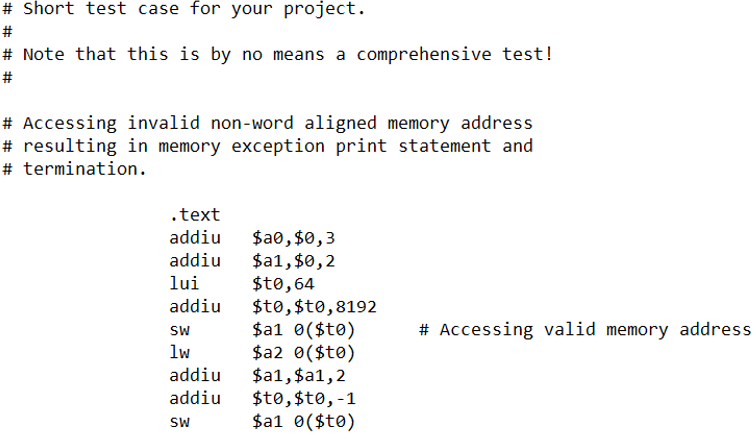
\includegraphics[width=130mm]{test_case1.png}
\end{center}
Test Case 2:
\begin{center}
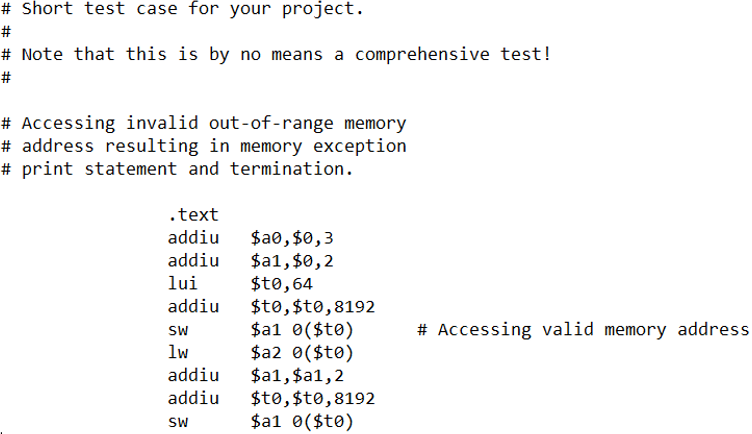
\includegraphics[width=130mm]{test_case2.png}
\end{center}
Test Case 3:
\begin{center}
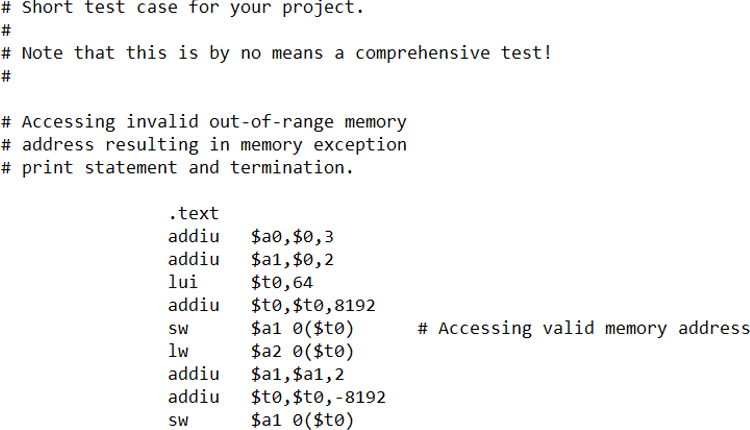
\includegraphics[width=130mm]{test_case3.png}
\end{center}
Test Case 4:
\begin{center}
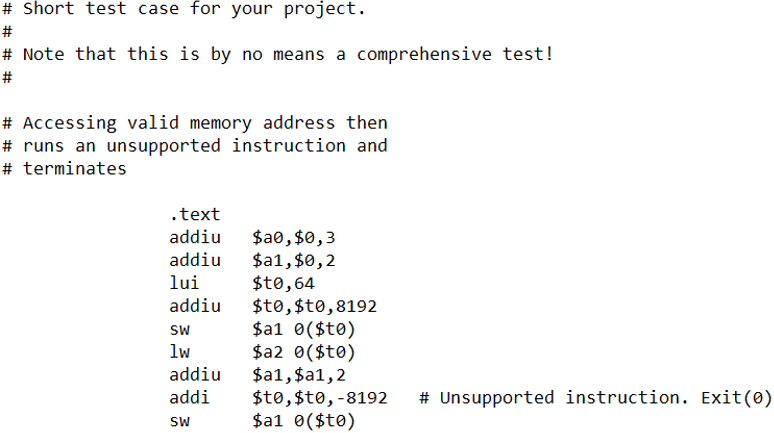
\includegraphics[width=130mm]{test_case4.png}
\end{center}
Test Case 5:
\begin{center}
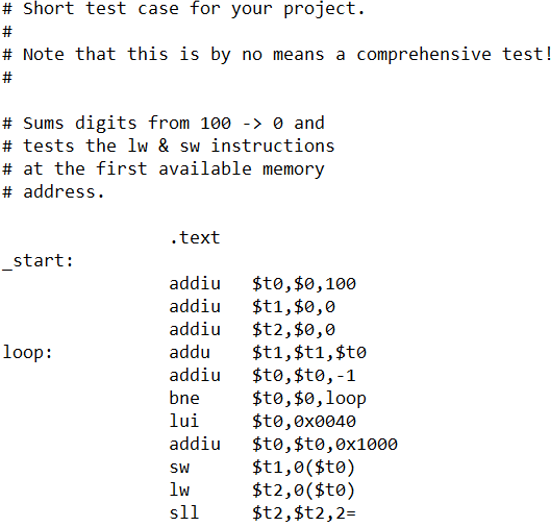
\includegraphics[width=100mm]{test_case5.png}
\end{center}
Test Case 6:
\begin{center}
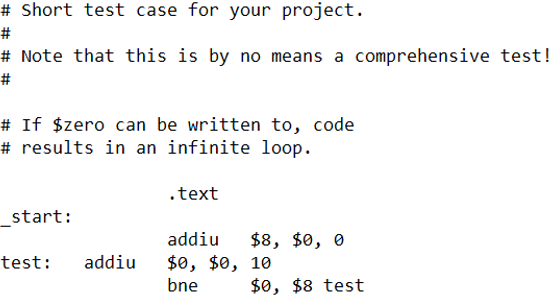
\includegraphics[width=100mm]{test_case6.png}
\end{center}
In this manner it is observable that the test case utilize a variety of procedural programming techniques, primarily loop iteration, jumps in memory referencing, and routine calls. As such the output for the cases are as follows:
\\
Output 1:
\begin{center}
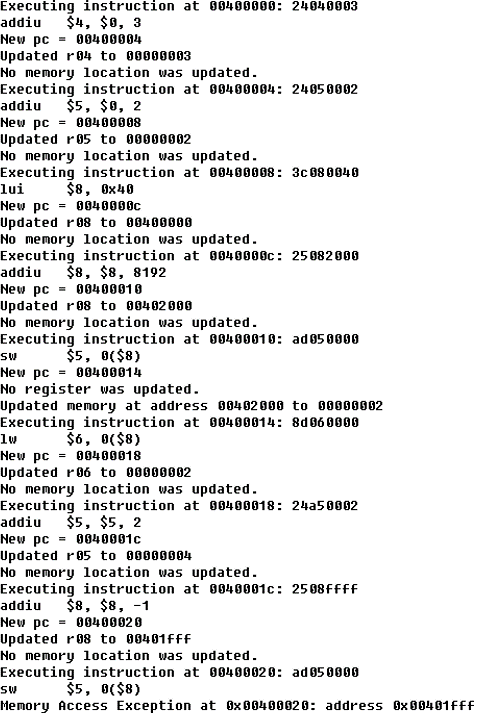
\includegraphics[width=100mm]{output1.png}
\end{center}
Output 2:
\begin{center}
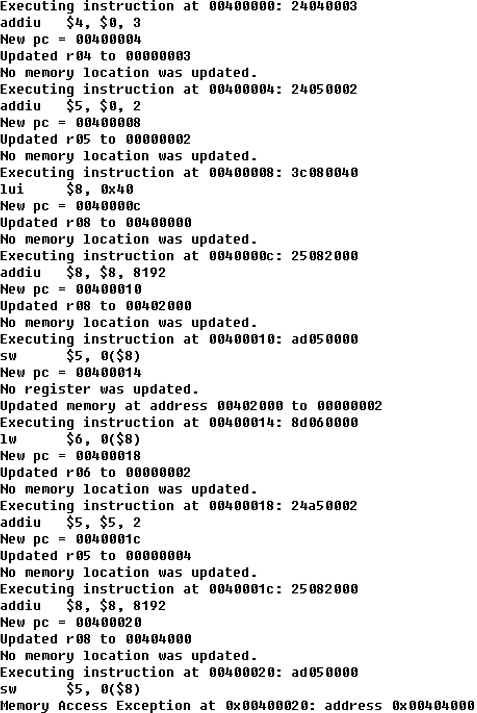
\includegraphics[width=100mm]{output2.png}
\end{center}
Output 3:
\begin{center}
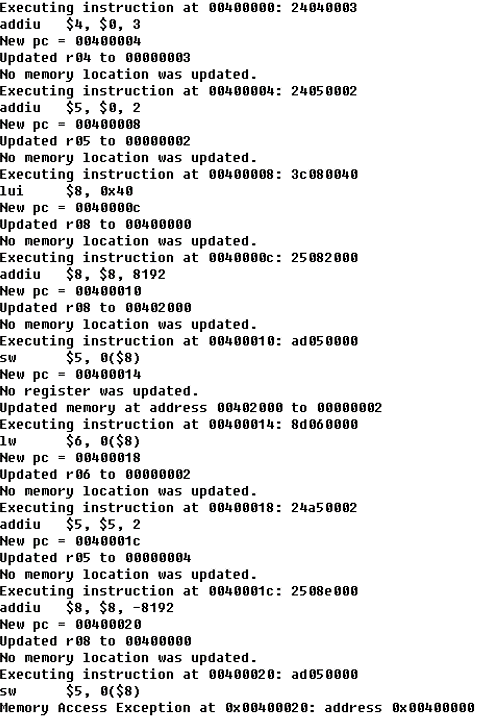
\includegraphics[width=80mm]{output3.png}
\end{center}
Output 4:
\begin{center}
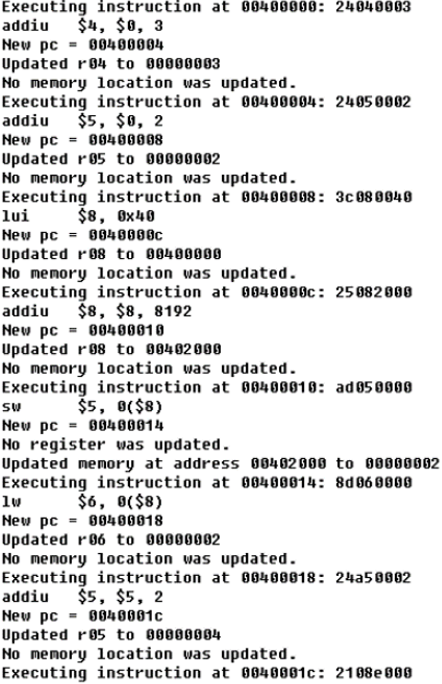
\includegraphics[width=80mm]{output4.png}
\end{center}
Output 5:
\begin{center}
\textit{omitted due to length, see} \textsc{test}\underline{\hspace{.3cm}}\textsc{cases} \textit{directory for further reference}
\end{center}
Output 6:
\begin{center}
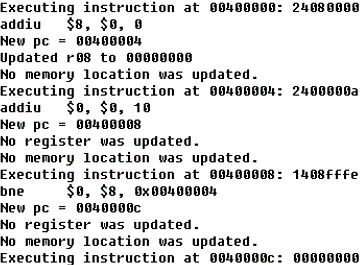
\includegraphics[width=70mm]{output6.png}
\end{center}
In essence these test cases provided an efficient, but not complete, set of both general and corner cases to test the validity of the simulated instruction interpreter system for \textsc{MIPS} in \textbf{\textit{C}}. The tests included:\begin{itemize}
\item infinite loops resulting from written \$\textsc{zero}
\item summing first 100 digits 
\item accessing invalid memory addresses to generate a memory exception
\item accessing out$-$of$-$range memory to generate a memory exception
\item running unsupported instructions
\item invoking the \textbf{\textit{C}} standard library \textsc{exit(...)} calls
\end{itemize} 
}
\end{document} 
